%%%%%%%%%%%%%%%%%%%%%%%%%%%%%%%%%%%%%%%%%%%%%%%%%%%%%%%%%%%%
%%% LIVECOMS ARTICLE TEMPLATE
%%% ADAPTED FROM ELIFE ARTICLE TEMPLATE (8/10/2017)
%%%%%%%%%%%%%%%%%%%%%%%%%%%%%%%%%%%%%%%%%%%%%%%%%%%%%%%%%%%%
%%% PREAMBLE 
\documentclass[9pt]{livecoms}
% Use the 'onehalfspacing' option for 1.5 line spacing
% Use the 'doublespacing' option for 2.0 line spacing
% use the 'lineno' option for adding line numbers. 
% Please note that these options may affect formatting.

\usepackage{lipsum} % Required to insert dummy text
\usepackage[version=4]{mhchem} 
\usepackage{siunitx}
\DeclareSIUnit\Molar{M}
\newcommand{\versionnumber}{1.3}  % you should update the minor version number in preprints and major version number of submissions.
%%%%%%%%%%%%%%%%%%%%%%%%%%%%%%%%%%%%%%%%%%%%%%%%%%%%%%%%%%%%
%%% ARTICLE SETUP
%%%%%%%%%%%%%%%%%%%%%%%%%%%%%%%%%%%%%%%%%%%%%%%%%%%%%%%%%%%%
\title{Best Practices for Transport Properties : v\versionnumber}

%Edward Maginn (ejmaginn), Richard Elliott, Sunny Hwang, Daniel Roe (GitHub: drroe), Rich Messerly (ramess101)

\author[1*,\authfn{1}\authfn{3}]{Edward Midname Maginn}
\author[2\authfn{1}\authfn{4}]{Daniel Midname Roe}
\author[3\authfn{1}\authfn{5}]{J. Richard Elliott}
\author[4\authfn{1}\authfn{6}]{Richard Alma Messerly}
\author[5\authfn{1}\authfn{7}]{Sunny Midname Hwang}
\affil[1]{Maginn's institution}
\affil[2]{Roe's institution}
\affil[3]{Elliott's institution}
\affil[4]{National Institute of Standards and Technology}
\affil[5]{Hwang's institution}

\corr{Maginn's email}{EM}  % Correspondence emails.  Second {} are the appropriate authors initials. 
\corr{Roe's email}{DR}
\corr{Elliott's email}{JRE}
\corr{richard.messerly@nist.gov}{RAM}
\corr{Hwang's email}{SH}

\contrib[\authfn{1}]{These authors contributed equally to this work}
\contrib[\authfn{2}]{These authors also contributed to this work}

\presentadd[\authfn{3}]{Maginn's Department, Institute, Country}
\presentadd[\authfn{4}]{Roe's Department, Institute, Country}
\presentadd[\authfn{5}]{Elliott's Department, Institute, Country}
\presentadd[\authfn{6}]{Thermodynamics Research Center, NIST, USA}
\presentadd[\authfn{7}]{Hwang's Department, Institute, Country}

%%%%%%%%%%%%%%%%%%%%%%%%%%%%%%%%%%%%%%%%%%%%%%%%%%%%%%%%%%%%
%%% ARTICLE START
%%%%%%%%%%%%%%%%%%%%%%%%%%%%%%%%%%%%%%%%%%%%%%%%%%%%%%%%%%%%

\begin{document}

\maketitle

\begin{abstract}
Please provide an abstract of no more than 250 words. Your abstract should explain the main contributions of your article, and should not contain any material that is not included in the main text.
\end{abstract}

List of people to contact: Peter Cummings, Richard Rowley, Joachim Gross, Raj Khare, Richard Sadus, Ioannis Economou, Jadran Vrabec, (any other Richards we can come up with)


\section{Outline}

Separate documents for:
\begin{enumerate}
	\item Equilibrium methods (self-diffusivity, viscosity) for liquids
	\item Non-equilibrium methods (self-diffusivity, viscosity) for liquids
	\item Methods for thermal conductivity
	\item Methods for ionic conductivity
\end{enumerate}

General outline of equilibrium methods of self-diffusivity and viscosity for liquids:
\begin{enumerate}
	\item Introduction
	\item Discussion of different methods within EMD (Green-Kubo, Einstein)
	\item General simulation set-up
	\item Diffusion
	\begin{enumerate}
		\item Brief discussion of why we recommend Einstein over Green-Kubo?
		\item Simulation setup that is specific to Einstein/diffusion
		\item Data analysis specific to Einstein/diffusion
		\item Common pitfalls for Einstein/diffusion
	\end{enumerate}
	\item Viscosity
	\begin{enumerate}
		\item Brief discussion of why we recommend Green-Kubo over Einstein?
		\item Simulation setup that is specific to Green-Kubo/viscosity
		\item Data analysis specific to Green-Kubo/viscosity
		\item Common pitfalls for Green-Kubo/viscosity
	\end{enumerate}
\end{enumerate}


\section{Introduction}

Transport properties describe the rates at which mass, momentum, heat or charge move through a given substance. They involve mean squared displacements (MSDs) of molecules as the system evolves dynamically. In general, these properties can be computed by equilibrium molecular dynamics (EMD) or by non-EMD (NEMD) methods. The equilibrium methods involve post-processing of a standard molecular dynamics (MD) trajectory while NEMD methods require modifications of the underlying equations of motion and/or boundary conditions of the system. Many codes such as LAMMPS and GROMACS have analysis tools that automatically estimate transport properties from an EMD or NEMD simulation, but there are often insufficient checks as to whether the actual underlying simulations are adequate for making these estimates. As Berk Hess has said in a forum post on using the GROMACS -vis option for calculating viscosity, ``...it will give nonsense unless you know exactly what you are doing''. For this reason, we highly recommend reviewing this list of existing resources:
\begin{enumerate}
	\item Text books:
	\begin{enumerate}
		\item \cite{Allen1987}, pages 58-64, 204-208, and 240-256
		\item \cite{Frenkel2002}, pages 87-90 and 509-523
		\item \cite{Leach2001}, pages 374-382
	\end{enumerate}
	\item Class notes
	\begin{enumerate}
		\item http://paros.princeton.edu/cbe422/md2.pdf
		\item http://paros.princeton.edu/cbe520/Transport.pdf
		\item https://engineering.ucsb.edu/~shell/che210d/Computing\_properties.pdf
	\end{enumerate}
	\item Published articles
	\begin{enumerate}
		\item \cite{Hess2002}
		\item \cite{Nieto2015}, pages 13139-13140
	\end{enumerate}
	\item Software manuals
	\begin{enumerate}
		\item GROMACS
		\item LAMMPS
	\end{enumerate}
\end{enumerate}
Most text books and class notes provide a thorough discussion of EMD/NEMD theory with little discussion of practical considerations. Review articles tend to focus on the numerical advantages and disadvantages of different methods but assume that the reader already understands the subtleties of each method. Furthermore, although the LAMMPS and GROMACS manuals describe some of the theory and implementation of these methods in their respective environments, the documentation is typically insufficient for someone not familiar with best practices for estimating transport properties. This document supplements the existing literature by providing a succinct checklist and common pitfalls. The purpose of this document is to improve the quality of published results and to cut down the time required to obtain meaningful and reliable results. %Citation -ramess101

\section{Equilibrium Molecular Dynamics (EMD) Routes to Transport Properties}

It is most convenient to consider compiling the transport properties as an implicit part of any equilibrium MD simulation. The added computational overhead is relatively small, especially for the self-diffusivity. The main caveat is that longer simulations than normal may be required to achieve reasonable averages. 

The general formula for computing a transport property via an EMD simulation is given as

\begin{equation} \label{eq:Green-Kubo}
\gamma = \int_{0}^{\infty}dt\langle\dot{\xi}(t)\dot{\xi}(0)\rangle
\end{equation}
where $\gamma$ is the transport coefficient and $\xi$ is the perturbation in the Hamiltonian associated with the particular transport property under consideration and $\dot{\xi}$ signifies a time derivative. Integrals of the form given by Equation \ref{eq:Green-Kubo} are known as “Green-Kubo” integrals. It is easy to show that an integrated form of Equation \ref{eq:Green-Kubo} results in an “Einstein” formula for the transport coefficient. Thus an equivalent expression for $\gamma$ is

\begin{equation} \label{eq:Einstein}
\gamma = \lim_{t\to\infty} \frac{\langle (\xi(t)-\xi(0))^2 \rangle}{2t}
\end{equation}

For self-diffusivity, $\xi$ is the Cartesian atom position and the time correlation function, $\dot{\xi}$, in Equation \ref{eq:Green-Kubo} is of the molecular velocities. For the shear viscosity, the integral in Equation \ref{eq:Green-Kubo} is of the time correlation of the off-diagonal elements of the stress tensor. For the thermal conductivity the integral is over the energy current, and for the electrical conductivity the integral is over the electric current. The relevant equations for self-diffusivity and shear viscosity are provided in Table \ref{tab:EMD_equations}.

% I think this table could be useful -ramess101

%\begin{table}[bt]
%	\caption{\label{tab:EMD_equations}Equilibrium molecular dynamics equations.}
%	% Use ``S'' column identifier to align on decimal point 
%	% ``l'' left aligns text in the column
%	% ``r'' right aligns text in the column
%	% ``c'' right aligns text in the column
%	% & separates columns, \\ ends the row.
%	
%	\begin{tabular}{l l l l l} 
%		\toprule
%		Property & $\gamma$          & $\xi$                        & Equation \ref{eq:Green-Kubo}    & Equation \ref{eq:Einstein}     \\
%		\midrule
%		Self-diffusion     & $D$ & $x$          & $\int_{0}^{\infty}dt\langle v_{x,i}(t) v_{x,i}(0)\rangle$    & $\frac{1}{2t}\langle (x_i(t)-x_i(0))^2 \rangle$   \\
%		Shear viscosity     & $\eta$       & $x v_y$           & $\beta V \int_{0}^{\infty}dt\langle P_{x,y}(t) P_{x,y}(0)\rangle$    & $\frac{m^2\beta}{2t}\langle (x_i(t)v_{y,i}(t)-x_i(0)v_{y,i}(0))^2 \rangle$  \\
%		Thermal conductivity      & $\lambda$      & $x E$              & $ \frac{k\beta^2}{V} \int_{0}^{\infty}dt\langle S_{x}(t) S_{x}(0)\rangle$    & $\frac{k\beta^2}{2Vt}\langle \left(x_i(t)(E_i(t)-\langle E \rangle)-x_i(0)(E_i(0)-\langle E \rangle)\right)^2 \rangle$  \\
%		\bottomrule
%	\end{tabular}
%$P_{x,y}(t) = \frac{1}{V} \sum_{i=1}^{N} \left( \frac{P_{x,i}(t)P_{y,i}(t)}{m} + x_i(t) f_{y,i}(t) \right)$
%\newline
%$S_{x}(t) = \frac{d}{dt} \sum_{i=1}^{N} \left( x_i(t) (E_i(t) - \langle E \rangle) \right)$.
%\end{table}

% Since this paper focuses on diffusion and viscosity I have removed conductivity. I also modified the equations somewhat. -RAM
%\begin{table}[bt]
%	\caption{\label{tab:EMD_equations}Equilibrium molecular dynamics equations.}
%	% Use ``S'' column identifier to align on decimal point 
%	% ``l'' left aligns text in the column
%	% ``r'' right aligns text in the column
%	% ``c'' right aligns text in the column
%	% & separates columns, \\ ends the row.
%	
%	\begin{tabular}{l l l l l} 
%		\toprule
%		Property & $\gamma$          & $\xi$                        & Equation \ref{eq:Green-Kubo}    & Equation \ref{eq:Einstein}     \\
%		\midrule
%		Self-diffusion     & $D$ & $\alpha$          & $\int_{0}^{\infty}dt\langle v_{\alpha,i}(t) v_{\alpha,i}(0)\rangle$    & $\frac{1}{2t}\langle (\alpha_i(t)-\alpha_i(0))^2 \rangle$   \\
%		Shear viscosity     & $\eta$       & $\alpha \dot{\beta}$           & $\frac{V}{k_bT} \int_{0}^{\infty}dt\langle P_{\alpha,\beta}(t) P_{\alpha,\beta}(0)\rangle$    & $\frac{m^2}{2k_bTVt}\langle (\alpha_i(t)\dot{\beta_i}(t)-\alpha_i(0)\dot{\beta_i}(0))^2 \rangle$  \\
%		\bottomrule
%	\end{tabular}
%\newline
%$P_{\alpha,\beta}(t) = \frac{1}{V} \sum_{i=1}^{N} \left( \frac{P_{\alpha,i}(t)P_{\beta,i}(t)}{m} + \alpha_i(t) \ddot{\beta_i}(t) \right)$
%\newline
%$\alpha$, $\beta = x, y, $ or $z$ coordinates
%\end{table}

\begin{table}[bt]
	\caption{\label{tab:EMD_equations}Equilibrium molecular dynamics equations.}
	% Use ``S'' column identifier to align on decimal point 
	% ``l'' left aligns text in the column
	% ``r'' right aligns text in the column
	% ``c'' right aligns text in the column
	% & separates columns, \\ ends the row.
	
	\begin{tabular}{l l l l l} 
		\toprule
		Property & $\gamma$          & $\xi$                        & Equation \ref{eq:Green-Kubo}    & Equation \ref{eq:Einstein}     \\
		\midrule
		Self-diffusion     & $D$ & $\r$          & $\int_{0}^{\infty}dt\langle v_{\alpha,i}(t) v_{\alpha,i}(0)\rangle$    & $ \lim_{t\to\infty} \frac{1}{2t}\langle |\r_i(t)-\r_i(0)|^2 \rangle$   \\
		Shear viscosity     & $\eta$       & $\alpha \dot{\beta}$           & $\frac{V}{k_bT} \int_{0}^{\infty}dt\langle P_{\alpha,\beta}(t) P_{\alpha,\beta}(0)\rangle$    & $ \lim_{t\to\infty} \frac{V2}{2k_bT}\langle (\alpha_i(t)\dot{\beta_i}(t)-\alpha_i(0)\dot{\beta_i}(0))^2 \rangle$  \\
		\bottomrule
	\end{tabular}
	\newline
	$P_{\alpha,\beta}(t) = \frac{1}{V} \sum_{i=1}^{N} \left( \frac{P_{\alpha,i}(t)P_{\beta,i}(t)}{m} + \alpha_i(t) \ddot{\beta_i}(t) \right)$
	\newline
	$\alpha$, $\beta = x, y, $ or $z$ coordinates
\end{table}


An important implicit assumption in the above equations is that the time over which these expressions are evaluated is much larger than the correlation time of the variable $\xi$. This assumption is often satisfied easily for simple liquids, where relaxation times are fast but becomes problematical for systems with sluggish dynamics. Obtaining reliable results with reasonable uncertainties can require simulations that are much longer than the longest relaxation times in the system, which are often unknown at the start of a simulation. Therefore, insufficient simulation time is a common pitfall in estimating transport properties.

Transport properties have to be estimated from the long-time integral of Equation \ref{eq:Green-Kubo} or the slope of Equation \ref{eq:Einstein}. Both methods involve some “judgment” on the part of the user and results can vary depending on where the slope is taken and for how long the integral is carried out. Some recent work has suggested some guidelines for how to compute an objective estimate of the viscosity using Equation \ref{eq:Green-Kubo}. Similar approaches for estimating other transport properties from Equations \ref{eq:Green-Kubo} or \ref{eq:Einstein} should be possible to develop. As no single best practice can be recommended for the region over which the slope or integral is calculated, it is important to justify how this decision was made. Furthermore, it is critical to quantify the degree of variability in the estimated property that arises from varying the time interval included in the data analysis. Precision in the final value is a key factor in selecting between the Green-Kubo or Einstein methods. For this reason, we emphasize the importance of proper data analysis and uncertainty quantification.

Although both Equation \ref{eq:Green-Kubo} (Green-Kubo) and Equation \ref{eq:Einstein} (Einstein) are theoretically rigorous, in practice one method is often preferred depending on the property being estimated ( $\propto \gamma$). In the case of self-diffusivity, we recommend the Einstein (MSD) approach. By contrast, for viscosity we typically recommend Green-Kubo, although for some systems the Einstein approach may be preferable.

\subsection{Checklist for Equilibrium Einstein Approach for Self-Diffusivity}

%I think that we should have this just as a general Einstein approach section and then if anything is specific to Self-Diffusivity we move it to a new section -ramess101

The Einstein approach is the most commonly used method for computing self-diffusivity. It is robust and we recommend this as the best approach.

\begin{enumerate}
	\item Ensemble - for a liquid solution, it is safest to run in the microcanonical (NVE) ensemble. %Although this may be the best practice, it appears to me that a large number of practitioners run their production simulations in the NPT ensemble. Should we point this out? I.e. should we say something like "although it is common to see values reported from the NPT ensemble..."? That way the reader will know why our recommendation seems to differ from what they find in the literature. -ramess101
	\begin{enumerate}
		\item Generally you want a self-diffusivity at a specified T and P. One needs to then equilibrate a system by first running an appropriate NPT simulation until equilibrium is well sampled (link to equilibration document). Using the average density computed from the NPT run, set the volume and run another NVT equilibration run. The last configuration from this run can then be used as input to start the NVE production run. The average pressure and temperature will need to be computed and should be close to (but not exactly the same) as the input to the original NPT run. These average pressures and temperatures must be reported along with the self-diffusivity. The user should generate multiple starting states that can be used to determine error estimation (see below).
		% Do we really just want the last configuration? Should we randomly select a configuration from production? Or a few configurations to run in parallel? Or somehow find an "average" configuration? My concern is just, what if the last configuration happens to be a higher energy sample (or lower probability if coming at it from a Monte Carlo point of view)? -ramess101
		\item For systems that require anisotropic pressure control (e.g. membranes etc), use of a barostat/thermostat that maintains the correct isothermal/isobaric ensemble (e.g. extended system, Langevin piston) is required.
	\end{enumerate}
	\item System size correction must be applied / finite size effects accounted for. See for example \cite{Yeh2004,Moultos2016}. This requires that the viscosity be calculated first or multiple simulations run with varying box sizes / number of molecules in order to estimate the infinite size limit of the self-diffusivity.
	\item Simulation length needed depends on number of molecules for which transport properties are desired. Fewer molecules = more simulation time and vice versa. Regardless, the simulation must be long enough so that the molecules are in the diffusive regime. One way of checking this is if the slope of a plot of ln(MSD) vs ln (t) = 1. Other heuristics are: is the MSD sufficiently large (larger than the square of the radius of gyration of the molecule at the low end, and larger than the square of half the box length at the high end).
	\item Ensure energy conservation (via adjusting time step, constraint tolerances, etc) (Link to document about initializing NVE in the right “ballpark.”) 
	\item Output frequency - how frequently do you write coordinates? Should be frequently enough so that you have around 1000 data points over the entire MSD.
	\item Use ``unwrapped coordinates'' of molecule center of mass to determine mean squared displacement; can also track all atomic coordinates and ensure consistency with center of mass.
	%Does ``unwrapped coordinates'' require an explanation? Do most open-source simulation packages have the option to track ``unwrapped coordinates''? -ramess101
	\item Compute the diffusion coefficient separately in each dimension, i.e. $D_{xx}$, $D_{yy}$, and $D_{zz}$. For a homogeneous system, $D_{xx}$, $D_{yy}$, and $D_{zz}$ should be equal. The variation in these values can be used for a rough estimate of the statistical uncertainty, although more rigorous methods for uncertainty estimation are recommended (see item 10).
	\item In order to obtain reliable estimates of D, it is important to consider how the linear regression is performed for the MSD with respect to time (Equation 2). Specifically, the time interval that is included in the regression can have a significant impact on the predicted value of D. We recommend that only the “middle” of the MSD be used in the fit. Short time must be excluded as it follows a ballistic trajectory, while very long time is excluded due to the increased noise. Currently, we are unaware of an objective approach for defining the “middle” region. Until such an approach exists, we recommend that the author reports how the region was selected and how much variability in D can be attributed to the choice of this region. 
	How do you fit the MSD (what time interval do you use?) Short time is ballistic trajectory; very long time you get noise, so you need to fit to the “middle” of the MSD. We need to define protocols for how to objectively define this. You should compute the uncertainty in the fit of the slope. Report how the line was fit and associated variables. Is there literature on this? We need to come up with a recommendation for how to do this objectively and consistently. 
	% If there is no published literature on the subject, rather than provide a recommendation, should we just present the issue that they need to be aware of? -ramess101
	% I think we should have a figure to help visualize this -ramess101
	\item Handling potential truncation: shifted force, shifted potential, cutoff, long range corrections. We need to come up with recommendations on this.
	\item Compute statistical uncertainty by running independent replicates (using multiple starting states from NPT run at desired temperature) and taking the standard deviation (what do the uncertainty people say?) How many replicates do we recommend? Link to Sampling/Uncertainty doc. Use Zwanzig/Szabo four-time correlation for MSD averaging….
	\item Multiple time origins used for MSD (block averaging) - is there a best practice?
	\item Calculating diffusion in membrane systems with PBC require some additional consideration, use of Saffman-Delbruck model: see http://pubs.acs.org/doi/abs/10.1021/acs.jpcb.6b09111, also http://dx.doi.org/10.1063/1.4932980
\end{enumerate}

FYI: Richard Elliot I developed a database for self-diffusivity that covered all experimental data from the literature as far as he could find. It is included as supporting information in Ind. Eng. Chem. Res. 2010, 49, 3411–3423. This paper provides a generalized correlation of the quantity rho*D (g/cm-s) of n-alkanes at all molecular weights, temperatures, and densities below the entanglement threshold. This semi-empirical correlation is used as the basis for correlating non-alkanes as well. Accuracy diminished for associating compounds, but experimental data were relatively few in number for associating compounds.

\subsection{Equilibrium Green-Kubo Approach for Self-Diffusivity}

Many of the same things apply as with the Einstein approach. Key differences:

\begin{enumerate}
	\item Need to write velocities instead of positions, and the frequency should be much higher because the integral of the velocity autocorrelation function decays rapidly. Recommend writing every 5 fs. 
	\item Integrate the VACF numerically, providing details of how this is done.
	\item Plot the running integral vs time. The data are best at short time and noise takes over at long times. Like with the MSD, a “cutoff” needs to be determined when you decide the integral has converged. Need objective measures for determining this.
	\item Averaging: independent simulations should be run, and each integral can be averaged together to obtain a smoothed integral. 
\end{enumerate}

\subsection{Checklist for Equilibrium Green-Kubo Approach for Viscosity}

Similar to self-diffusivity, EMD for viscosity is straightforward but its reliability compared to experimental data has not been evaluated with a comprehensive database. Many more experimental data are available for viscosity than for self-diffusivity. Anecdotal studies with small databases show encouraging results, but deviations from experiment can range from 5-35\% even when results are said to be “good.” Nieto-Draghi et al. provide a useful review of the status quo \cite{Nieto2015}. EMD may deviate 2x more than NEMD from experimental data; hydrogen bonding throws in complications that may require empirical corrections. 

% I don't think we want to talk about comparison to experimental data. We are not really concerned about if diffusivity or viscosity are accurately predicted relative to experiment, we just want to present the best methods for obtaining reproducible/honest results. In addition, you can predict viscosity more accurately if you parameterize your force field for such a purpose. -ramess101

% I am unaware of this - can a citation be given? -ejmaginn

\begin{enumerate}
	\item Ensemble: NPT is not recommended. NVE is ideal; NVT has been used with success.
	\item Finite size effects: Figures \ref{fig:MoultosFig3}-\ref{fig:ZhangFig9} from Moultos et al. and Zhang et al., respectively, suggest that finite size effects are not significant above a threshold size. More work needs to be done to verify this. We recommend that users look for system size effects by plotting the viscosity with respect to $N^{-1/3}$, where $N$ is the number of molecules. The range of $N$ should span an order of magnitude or, if this is computationally intractable, at least a factor of two. If a linear trend is observed with respect to $N^{-1/3}$, the infinite system size viscosity can be extrapolated as the intercept from a linear regression.
	% Should we recommend how much to vary the system size? In other words, varying the size from 200 to 250 is probably not very informative. But varying the size from 200 to 400 to 800 to 1600 will probably show you if there is a trend. So should we recommend "several" different system sizes that vary by a factor of 2 or greater? Also, normally the plot has 1/N^(some power) as the horizontal axis, where the power might have a theoretical value. These plots are nice since N=infinity corresponds to the vertical axis. I think we should mention this. -ramess101
	\item Simulation length: overall you need about 10X more data to compute viscosity than diffusivity, since viscosity is a collective property.
	% Do we have any literature to support this? -ramess101
	\item Output frequency should be high (every 5-10 fs); this needs to be checked for the particular system 
	% The 5-10 fs is redundant with what we have in diffusivity section -ramess101
	\item GK method works for fluids with relatively low viscosity (less than 50 cP). Higher viscosity systems are extremely difficult to compute with GK (NEMD methods are often preferred in this case).
	\item Sufficient simulation time for “4-5 molecular rotations” on average. Averaging over multiple simulations with analytic fitting of integral provides a good way of smoothing noise and provides an objective means of determining the viscosity \cite{Zhang2015}.
    % I think this point of averaging multiple simulations is important enough to merit its' own discussion
	\item Perform independent replicate trajectories (i.e. different initial configurations or random seed to initialize velocities). The primary advantage of performing replicates is the computational speed-up. Figure BLANK taken from Payal et al. \cite{Payal2012} demonstrates that an average of 10 replicate simulations of 2 ns length converges to the same value as a single 4 ns simulation. Since these replicates can be performed in parallel the computational time is reduced by a factor of two, in this example. However, Figure BLANK, taken from Zhang et al., demonstrates that if the length of each independent trajectory is too short the viscosity will not converge to the correct value, regardless of how many replicates are used. 
	\item The number of replicates used in literature varies widely. Payal et al. used 10 replicates whereas Zhang et al. performed a systematic investigation of the minimal number of replicates required for convergence. They observed that a value of 30-40 replicates was statistically equivalent to 100 replicates for their system. However, the necessary number of replicates depends on the system. Specifically, the most important factors are the compound, the temperature, the number of molecules, and the simulation time.  In addition, replicates can provide a more rigorous uncertainty assessment. We recommend bootstrapping the uncertainties by randomly sampling which replicates are included in the average and data analysis procedure. An example of the distribution obtained from bootstrapping is found in Figure BLANK. Furthermore, because the uncertainty is inversely proportional to the square root of the number of replicates (see Figure 7 of Zhang et al. and Figure 8 of Ma et al.), increasing the number of replicates is a simple, fast, and direct way to reduce the uncertainty to the desired level.
	\item Report how the viscosity was estimated from the ``running integral''. For example, it is a common practice to report an average that is obtained over a region of time. It is important to explain how this region of time was selected (i.e. visual inspection, test of convergence, etc.) and to quantify how much the estimated viscosity would change if the region over which the average is calculated was modified. Alternatively, we recommend fitting an analytic function to the ``running integral''. For example, Zhang et al. recommended fitting the ``running integral'' to a double-exponential function. In this case, it is important to include a description of how the fit is performed, i.e. the objective function, weighting model, range of data included, etc. Zhang et al. recommend that the data be weighted by the inverse of the standard deviation with respect to time. The form of their weighting model is $w \propto t^{-b}$, where $w$ is the weight, $t$ is the time, and $b$ is the weighting exponent. If such a model is utilized, we recommend that the author quantifies uncertainty in the estimated viscosity due to the value of $b$, the weighting exponent. For example, Zhang et al. compared two different values of $b$ in Figures 7, 12, and 13. They also suggest that to improve the fit a cut-off time be implemented. They provide a heurestic that the cut-off time be that when the standard deviation is 40\% the plateau value. Regardless of how the cut-off is determined, it is important to quantify the degree to which the estimated viscosity depends on this parameter. For example, Zhang et al. reported that a cut-off at 30\% or 20\% decreased viscosity by 0.8\% and 6.1\%, respectively. The variability that is observed depends strongly on the system. If such a method is employed, we recommend that the author demonstrate the cut-off time dependence. For example, plots of the estimated viscosity with respect to the weighting exponent and cut-off time, such as those shown in Figure BLANK, provide a quantitative measure of confidence in the viscosity value.  
	\item Force fields: systematic consideration of the intra- vs. inter- molecular potential models; UA, vs. AUA vs. EA differences may be significant. For charged systems, polarizable force fields might be needed to get accurate results. Some studies have suggested that united-atom models are not capable of accurately reproducing viscosity and, therefore, anisotropic-united-atom or all-atom models are needed \cite{Allen1987,Payal2012,Mondello1997}. However, other studies have shown that with the appropriate tuning of the united-atom force field parameters viscosity can be accurately predicted without significant deprecation of other properties \cite{Gordon2006}.
	
	\begin{figure}[htb!]
		\centering
		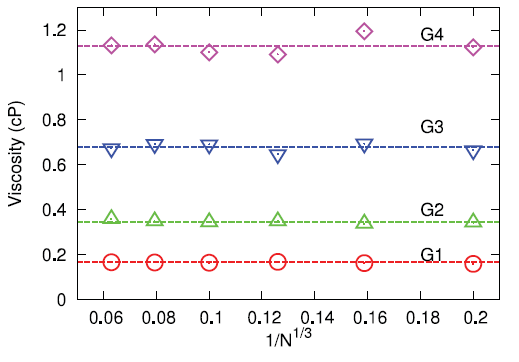
\includegraphics[width=3.2in]{figures/MoultosFig3.png}
		\caption{}
		\label{fig:MoultosFig3}
	\end{figure}

	\begin{figure}[htb!]
		\centering
		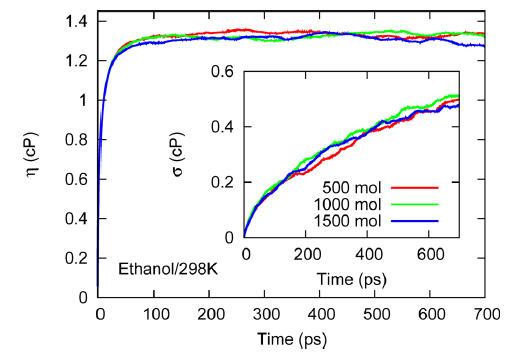
\includegraphics[width=3.2in]{figures/ZhangFig9.png}
		\caption{}
		\label{fig:ZhangFig9}
	\end{figure}
	
\end{enumerate}

\subsection{Equilibrium Einstein Approach for Viscosity}

Similar to the Green-Kubo approach, the key to obtaining precise estimates of viscosity with the Einstein approach is to average multiple replicate simulations. The viscosity with respect to time is estimated from the slope of the Einstein integral. Thus, the average of replicates can be performed in one of two ways. The first option is to calculate the viscosity with respect to time for each replicate and then average the replicates. However, this approach results in large fluctuations, similar to the Green-Kubo approach. The second, and recommended, method is to average the Einstein integral of the multiple replicates. The resulting Einstein integral is often linear over a large time interval if sufficient replicates are used. Subsequently, the slope is determined from this average Einstein integral. In general, the initial time should be discarded. Since the Einstein relation is valid in the limit of infinite time, it is common to fit the slope at long time. However, it is also common to fit the slope to an intermediate time interval. We recommend that the author explain why the slope was calculated using a given time interval and how much variability is introduced if a different region is selected. Fortunately, with sufficient replicate simulations the slope tends to be fairly constant over short, intermediate, and long time intervals. The number of replicates needed has not been rigorously investigated as it has for the Green-Kubo approach. For this reason, we recommend creating a plot of viscosity with respect to number of replicates to determine when sufficient replicates have been simulated. It is our experience that the number of replicates is similar to that for Green-Kubo. As recommended for Green-Kubo, we also recommend bootstrapping the uncertainty by randomly sampling which replicates are averaged for calculating the slope.

Hess claims that the Einstein relation is more convenient than Green-Kubo for viscosity because ``inaccuracies in the long time correlations can be ignored by only considering integral over shorter times.'' 
%What do we want to make of this claim? -RAM

\section{Non-Equilibrium Molecular Dynamics (EMD) Routes to Transport Properties}

NEMD methods require the use of a modified Hamiltonian to drive the system away from equilibrium. By monitoring the response of the system in the limit of a small perturbation, the transport coefficient associated with the perturbation can be calculated [I would cite Evans and Morriss here]. The basic idea behind the technique is that a system will respond in a linear fashion to a small perturbation. The following linear response theory equation is applicable in this limit

\begin{equation}
J = -L \nabla X
\end{equation}

where J is the response, X is the perturbation and L is the transport coefficient. For example, eq 3 takes the following form for the viscosity

\begin{equation}
j_y(p_x) = -\eta \frac{\partial v_x}{\partial y}
\end{equation}
where $j_y(p_x)$ is the momentum flux, $\frac{\partial v_x}{\partial y}$ is the velocity gradient or shear rate and $\eta$ is the shear viscosity.  The most widely used NEMD approach for viscosity calculations is the so-called “SLLOD” algorithm [cite] in which a shear rate is imposed on the system and the resulting stress is computed. The shear viscosity is found at a given shear rate from the ratio of the off-diagonal components of the stress tensor to the shear rate. This gives a shear-rate dependent viscosity, which must be extrapolated to a zero shear rate in order to estimate the Newtonian shear viscosity. This points out two issues with getting accurate Newtonian shear viscosities from NEMD: 1) Ensuring the off-diagonal stress tensor average is converged for a given shear rates and 2) Using a reliable method for extrapolating the shear-dependent viscosity to a zero shear rate. 

As noted above, it is possible to obtain transport coefficients using equilibrium methods via Green-Kubo (eqn 1) and Einstein (eqn 2) approaches as well as non-equilibrium (eqn 3) methods. Which approach a user chooses depends on the property and, to some extent, the preference of the user. Each property and method requires a slightly different checklist, and so we have chosen to break these lists out into the property computed and whether equilibrium or non-equilibrium methods were used.

\section{Non-Equilibrium SLLOD Approach for Viscosity}

In this method, a shear is imposed on the fluid through sliding Lees-Edwards boundary conditions. The resulting stress is computed and related to the shear viscosity by the standard Newtonian viscosity relation.

\begin{enumerate}
	\item Ensemble: Due to the sliding boundary conditions, energy is added to the system and so a thermostat must be used to remove this energy. Thus NVT must be used.
	\item The computed viscosity will be shear rate dependent; typical shear rates are much higher than what is obtainable experimentally, so a series of simulations must be run at different shear rates. Extrapolation to zero shear rate is done to estimate the Newtonian viscosity. There is no formal theoretical method for making this extrapolation, but the Carreau model \cite{Hieber1992,Kioupis2000}, has often been used.
	\item User selects a series of shear rates to impose; some trial and error is required to ensure that the rate is high enough to get a stress “signal” but low enough so that extrapolation to zero shear can be obtained. Rule of thumb: the inverse shear rate where shear thinning starts roughly corresponds to the rotational correlation function time constant of the longest molecular axis.
	\item Parametric studies should be done varying the thermostat time constant to ensure proper temperature profiles. 
	\item It is possible to implement this method with “real walls”, mimicking an experimental viscosity measurement. In this case, the walls are thermostatted and a nature temperature profile evolves.
\end{enumerate}

\section{Reverse Non-Equilibrium Approach for Viscosity}

This method is like the opposite of SLLOD; the stress is imposed by swapping velocities of molecules between layers or slabs, and the resulting shear profile is measured. The basics of the method are shown in Fig. 1. This is much easier to compute, but requires more computational infrastructure. The method \cite{Muller1999} has been implemented in LAMMPS \cite{LAMMPS} and critically compared to EMD and standard NEMD methods for simple Lennard-Jones systems \cite{Tenney2010}. 
 
\section{Thermal Conductivity}

Molecular simulation methods for thermal conductivity are fairly underdeveloped, perhaps owing to the radiative heat transfer issue.

Checklist for calculating ionic conductivity. This is a hard property to compute. Once again, NEMD and EMD methods need to be treated separately. NEMD methods (imposing electrical field and measuring fluxes) might be 

For thermal conductivity of solids, beware of isotope effects, radiation, electrons,... other deviations from classical mechanics. 


\section{Ionic Conductivity}

Probably recommend EMD approaches similar to GK viscosity. NEMD methods are perhaps easiest to apply for this property.

\section{Transport Diffusivity}

Unlike self-diffusivity, this is a collective property like viscosity. Can be computed with EMD and NEMD methods. Need to modify these checklists for this property. 

\begin{enumerate}
	\item Darken correction
	\item DCV GCMD
	\item External Field NEMD
\end{enumerate}

\section{Other things...}

In the case of self-diffusivity, it is straightforward to obtain reliable estimates through the Stokes-Einstein relation. In the case of viscosity, EMD signal-to-noise ratio is not as favorable and Green-Kubo relations may be preferable. One way of enhancing signal-to-noise is through NEMD, but care must be taken when extrapolating to zero shear. All fluids are shear-thinning if the shear rate is high enough, and NEMD methods tend to exert remarkably high shear rates. Thermal conductivity is simpler than the other two in the sense that it approaches an asymptote in the long chain limit, whereas the scaling changes with molecular weight for diffusivity and viscosity when one surpasses the entanglement threshold (roughly 1500 amu for olefin polymers). Unfortunately, molecular dynamics alone cannot accurately characterize the thermal conductivity at low density. Apparently radiative heat transfer may be important in these cases, with deviations around 30\% from MD results. MD results for spheres are consistent with the Chapman-Enskog relations in the low density limit for all three properties.

%Do you mean the Einstein relation and not Stoke-Einstein? -ramess101

\section{Acknowledgments}

Funder and other information can be given here.

%\nocite{*} % This command displays all refs in the bib file
\bibliography{transport_properties}

%%%%%%%%%%%%%%%%%%%%%%%%%%%%%%%%%%%%%%%%%%%%%%%%%%%%%%%%%%%%
%%% APPENDICES
%%%%%%%%%%%%%%%%%%%%%%%%%%%%%%%%%%%%%%%%%%%%%%%%%%%%%%%%%%%%

\end{document}